\section{Production of hyperon resonance}

The Quark Model, proposed independently by Murray Gell-Mann and Yuval Ne'eman in 1964 \cite{cite:gellmann}, enables the classification of hadrons in terms of their constituent quarks. In this model, the lighter mesons and baryons are representations of an SU$_{f}$(3) group, whose fundamental representation is the three dimensional vector (u, d, s). These are the three lighter quarks whose characteristics are reported in Table ref{table:quark}. 

\begin{table}[h!]
\centering
\begin{tabular}{lclclc|c|}
\hline
Light flavor &   d  & u  & s \\
\hline \noalign{\smallskip}
Baryon number (B) &  +1/3     & +1/3  &  +1/3\\
Electric charge (Q) &   -1/3     &  +2/3 &   -1/3 \\
Isospin (I)               &   -1/2     &  +1/2 &     0\\
Strangeness (S)     &     0   & 0 & -1\\
mass (\mmass)   &    2.3$_{-0.5}^{+0.7}$    & 4.8$_{-0.3}^{+0.5}$  &  95$\pm$5\\
\hline\noalign{\smallskip}
\noalign{\smallskip}
\end{tabular}
\caption{Quantum numbers and masses associated to the three lighter quarks: u, d and s}\label{table:quark}
\end{table}

The hadronic state are obtained from the decomposition of the following scalar products of the fundamental representations of the group: \\

Meson (q$\bar{q}$) :  3 $\bigotimes$ $\bar{3}$ =  1 $\bigoplus$ 8 \\

Baryon (qqq) : 3 $\bigotimes$ 3 $\bigotimes$ 3  =  10$_{S}$ $\bigoplus$ 8$_{M}$ $\bigoplus$ 8$_{M}$ $\bigoplus$ 1$_{A}$ \\

For the baryons without $c$ or $b$ qaurk, flavor and spin may be combined in an approximate flavor-spin SU(6), in which the six basic states are d $\uparrow$, d $\downarrow$, $\cdot$ $\cdot$ $\cdot$, s $\downarrow$ ($\uparrow$, $\downarrow$ = spin up, down). Then the baryons belong to the multiplets on the right side of \\

6 $\bigotimes$ 6 $\bigotimes$ 6  =  56$_{S}$ $\bigoplus$ 70$_{M}$ $\bigoplus$ 70$_{M}$ $\bigoplus$ 20$_{A}$ \\

Here, the 56 representation can be decompose in an octet ($J^{P}$ = 1/2$^{+}$) and a decuplet ($J^{P}$ = 3/2$^{+}$), as can be seen in Figure \ref{fig:octet} and Figure \ref{fig:decuplet}.

\begin{figure}[htbp]
\begin{center}
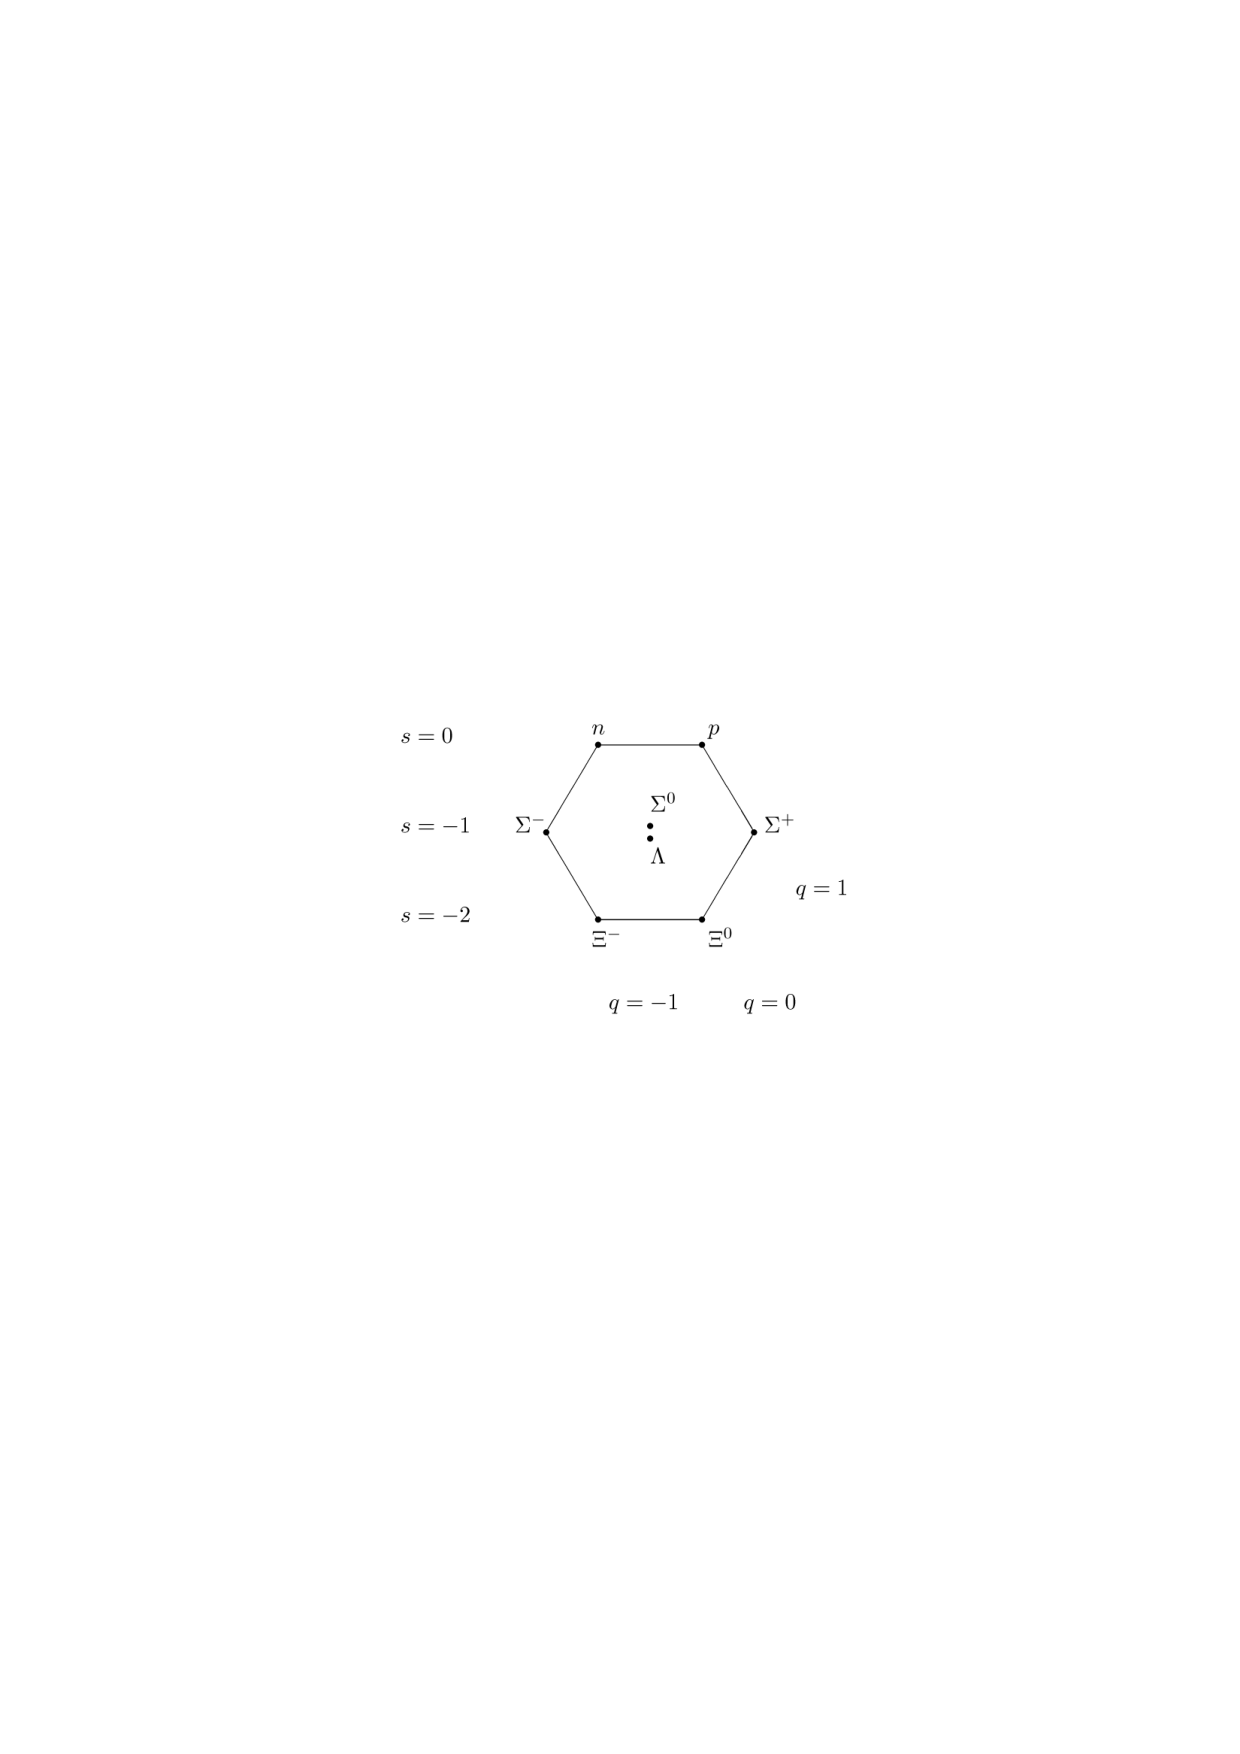
\includegraphics[width=10.cm]{./Version1/FigChapter3/Octet}
\caption{ The $J^{P}$ = 1/2$^{+}$ ground state baryon octet}
\label{fig:octet}
\end{center}
\end{figure}

\begin{figure}[htbp]
\begin{center}
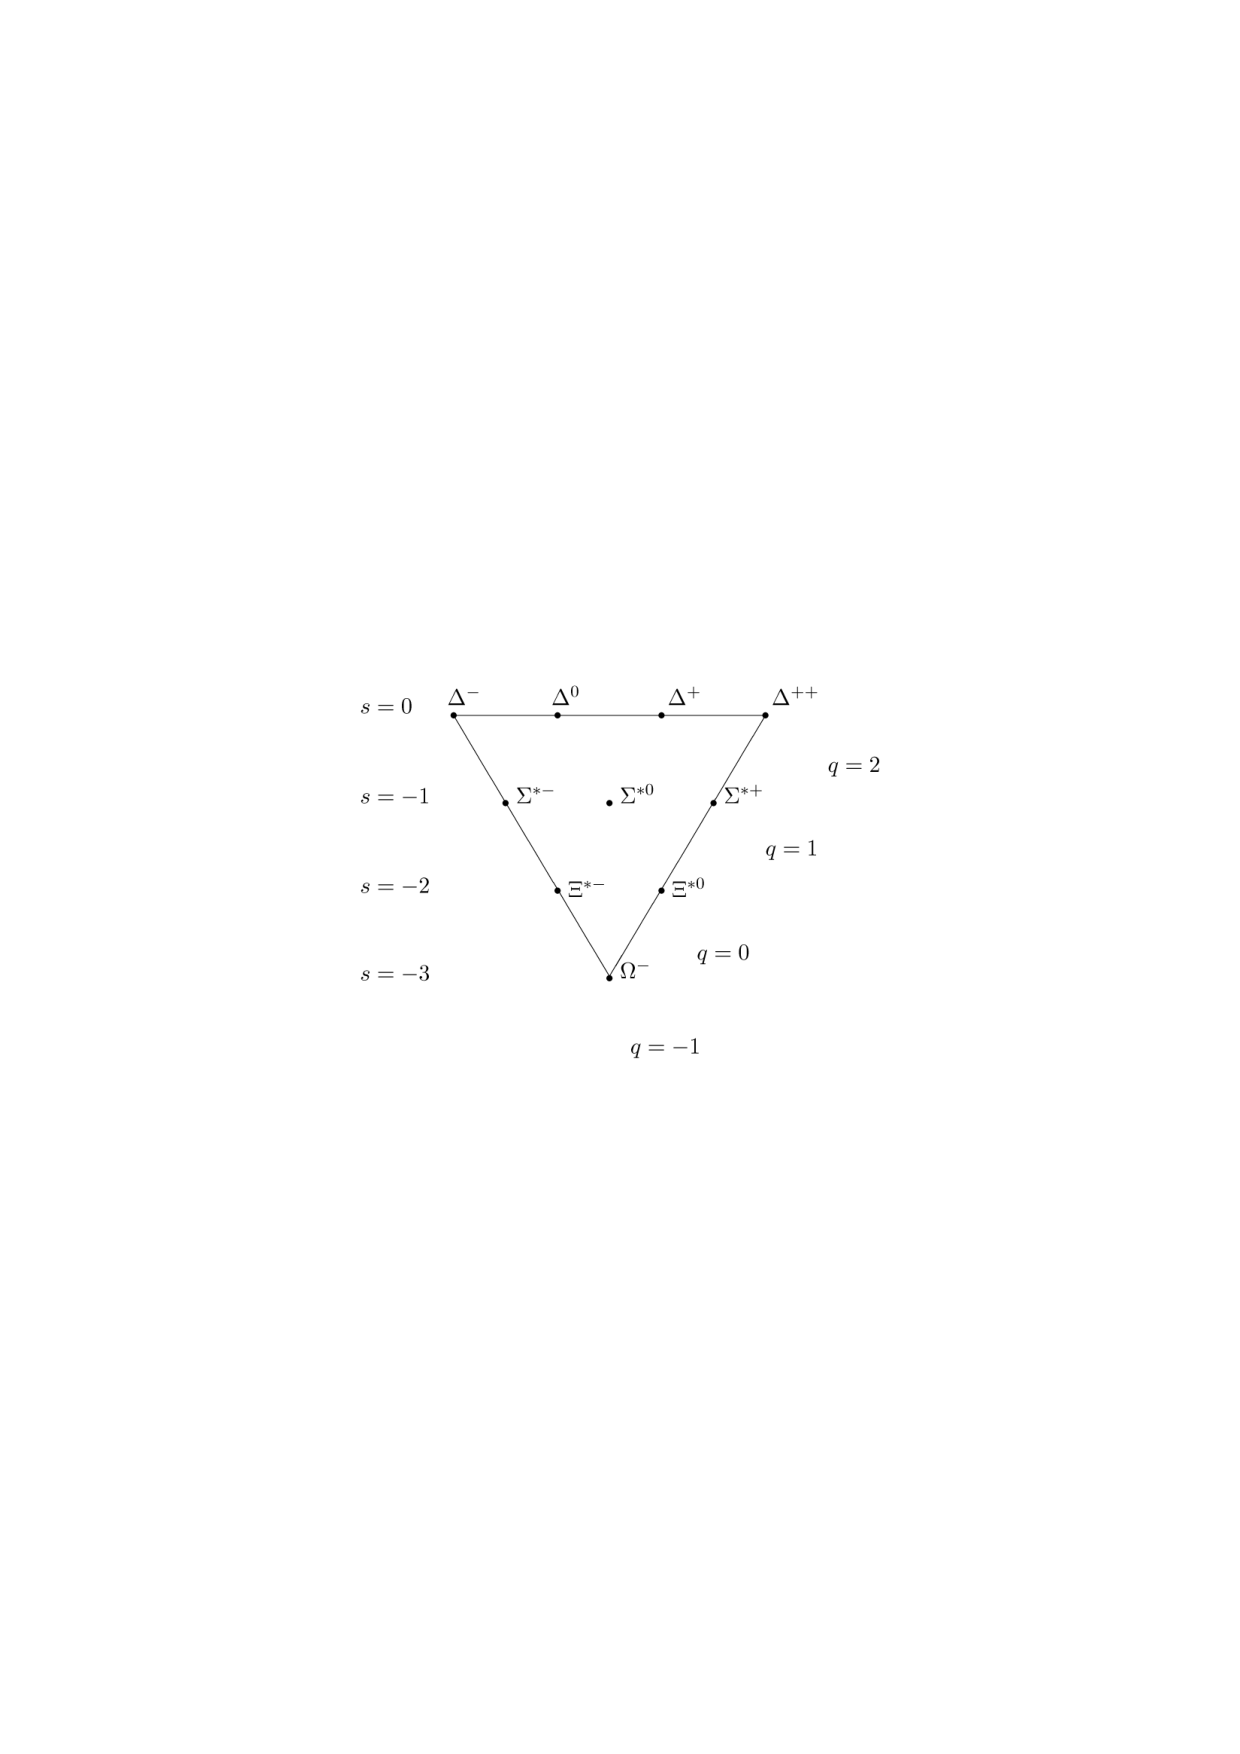
\includegraphics[width=10.cm]{./Version1/FigChapter3/Decuplet}
\caption{ The $J^{P}$ = 3/2$^{+}$ baryon decuplet}
\label{fig:decuplet}
\end{center}
\end{figure}

Among these hadrons, the special family of particles that contain at least one strange quark but not heavier quarks (like charm or bottom), are called hyperons. These are: the $\Lambda$(uds), the triplet $\Sigma^{+}$(uus), $\Sigma^{0}$(uds), $\Sigma^{-}$(dds), the doublet $\Xi^{-}$(dss), $\Xi^{0}$(uss) and the $\Omega$(sss) and the corresponding antiparticles. $\Xi$ and $\Omega$ are the only hyperons containing more than one strange quark, hence they are called multi-strange baryons. 
Resonances shown in Figure ref{fig:decuplet} having * with its name (e.g. X*$^{\pm}$) are particles which have higher mass than the corresponding ground state particle with the same quark content. 

Different resonances having various lifetimes (Table \ref{table:rsnptl}) can be used as tool to explore different stages of the fireball expansion as discussed in section \ref{sec:hi}. In order to have insight on the role of the re-scattering effect between the freeze-out phases, it is important to measure the ratio between resonances and stable hadrons and  compare it with different lifetimes. 


\begin{table}[h!]
%\centering
\begin{center}

\begin{tabular}{|c|c|c|c|c|c|c|clc|c|c|}
\hline
Particle & $\rho$(770) & $\Delta$(1232) &K*(892) & $\Sigma$(1385) &$\Lambda$(1520) & $\Xi$(1530)& $\Phi$(1020)\\
\hline
Lifetime[c$\tau$] &  1.3 fm &1.7 fm & 4.0 fm& 5.5 fm& 10.3 fm & 22 fm& 46 fm\\
\hline
\end{tabular}
\caption{Lifetime of hadronic resonances}\label{table:rsnptl}
\end{center}
\end{table}



In the following, a general overview of the role of the strange quark within the QGP studies with heavy-ion collisions is given.
%First of all, no net strangeness is present in the colliding objects before collision. Indeed, both the nucleons, proton and neutron, contain only u and d quarks among their valence quarks. All the net strangeness present in the final states (particles) is then created during the collision, and therefore the s quark plays an interesting role in the study of particle production.
And importance of the measurement of resonance is explained as probe of properties in the duration of hadronic phase from the chemical($T_{ch}$) to the kinetic freeze-out($T_{kin}$). 



\subsection{Strange quark and hyperons}
  
The original interest in the strangeness in the context of the QGP comes from an idea by Johann Rafelski and Berndt M$\ddot{u}$ller. In 1982, they suggested a possible signature for the formation of a QGP in a heavy-ion collision \cite{cite:strangeness}. The key argument, at a fixed collision energy, rests on the different production mechanism of the s quark within two different systems:
\begin{description}
\item[1. Hadron Gas (HG)], where the degrees of freedom are the hadronic ones, as quark and gluons are confined.
The great abundance of pions in the HG suggests to consider the production of strange particles from the reaction between them.
Direct production can be observed with $\pi$ + $\pi$ $\rightarrow$ $\pi$ + $\pi$ + strange hadron + antiparticle, considering the baryon and strange number conservation. This means that, in order to create the strange particle and anti-particle at once, the reaction threshold (energy needed to produce mesons or baryons) corresponds to tow times the rest mass of the hadrons. (2230 MeV for $\Lambda$+$\bar{\Lambda}$, 2642 MeV for $\Xi$+$\bar{\Xi}$. 3344 MeV for $\Omega$+$\bar{\Omega}$)

%In the case of indirect production, the thresholds are lower. In this case, one would have two reactions in a sequence, starting with the production of lighter hadrons (? + N ? K + ?) and followed by a re- action of these intermediate products to produce the heavier hadrons (?+? ? K+? and ?+? ? K+?). In this case the combined thresh- olds for the production of a ? is (535 + 565) MeV = 1100 MeV and for the production of an ? is (535 + 565 + 710) MeV = 1810 MeV.

\item[2. QGP], where the degrees of freedom are partonic ones, with quarks and gluons free with respect to each other. The high gluon density gives the possibility to have new production mechanisms abreast the usual quark-pair annihilation which are the gluon fusion processes. It becomes the dominant process of $s\bar{s}$ pairs creation. In these reactions the energy threshold is equal to the naked mass of the two strange quarks $\approx$ 2 $\cdot$ 100 MeV.
\end{description}


%The mass of the hadrons is only partly due to the mass of the constituent valence quarks.

The quarks can not be seen directly due to the strong interaction which keeps them confined. Once they are free, as in a QGP, the quarks recover their bare masses. (Note that, only the part of mass of hadron comes from the mass of the constituent quarks.)
It was predicted that, if the QGP is formed, an enhancement of the strange quarks should occur, because the production of $s\bar{s}$ pairs becomes easier due to the lower energy needed as explained above. When the QGP cools down, these strange quarks eventually recombine into hadrons favoring also an enhancement of the number of strange hadrons. This effect is larger for hadrons with higher strangeness, with the following scaling for the number type: \\
Ordering in QGP: $N_{\Omega} >  N_{\Xi} > N_{\Lambda}$

where $N_{\Omega}$, $N_{\Xi}$, $N_{\Lambda}$ are the number of produced $\Omega$, $\Xi$ and $\Lambda$. A certain enhancement of strange hadrons can occur also in a hadron gas system, but the processes of hadronisation in this case are relatively easy for K and  $\Lambda$. and progressively harder for hadrons with higher strangeness, hence the relation would be: \\
Ordering in HG: $N_{\Omega} <  N_{\Xi} < N_{\Lambda}$.

The measurement of multi-strange hadrons in heavy-ion collisions with respect to small collisions is considered to be a signature of the formation of the QGP and it was observed at SPS, RHIC and LHC. \cite{cite:strangePbPb}


\begin{figure}[htbp]
\begin{center}
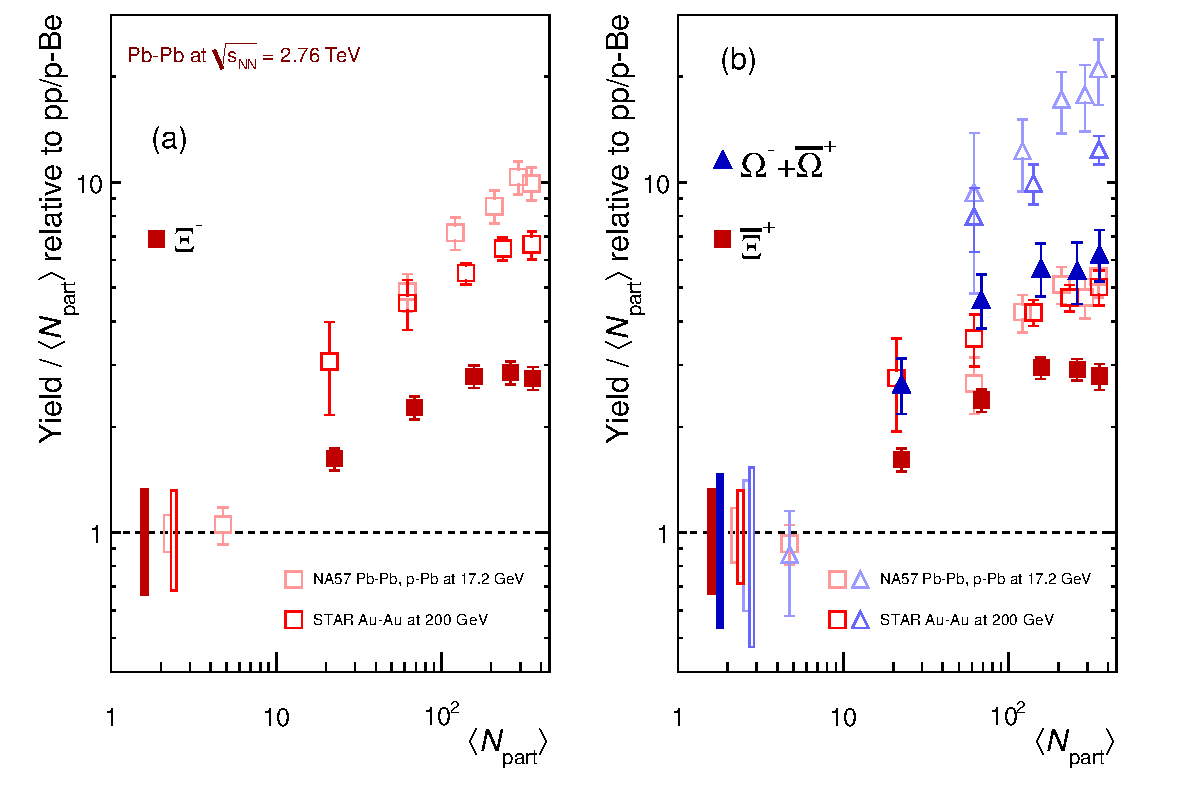
\includegraphics[width=12.cm]{./Version1/FigChapter3/MultdNdy}
\caption{Integrated yield relative to small system (pp or p--Be) as a function of the mean number of participants  $\langle N_{part}\rangle$ in the rapidity range $\arrowvert y \arrowvert<$0.5. The results from ALICE are presented as full symbols, RHIC and SPS data are shown as open symbols. Boxes on the dashed line at unity represent statistical and systematic uncertainties on the pp or p-Be reference.}
\label{fig:dNdy}
\end{center}
\end{figure}


The measured enhancement factors of baryons with increasing strangeness content are reported in Figure \ref{fig:dNdy} as a function of the mean number of participants, $\langle N_{part}\rangle$, compared with measurements at SPS and RHIC. 
As shown in the Figure \ref{fig:dNdy}, the enhancement increases with $\langle N_{part}\rangle$ which is variable to be comparable to the centrality in Pb--Pb collisions and the effect is more pronounced for particle with larger strangeness content. If one consider the collision energy dependency, the comparison with measurement from the previous experiment shows that the relative enhancements degrease with increasing energy.  An explanation of this behavior is given in terms of a statistical model, with canonical strangeness conservation. 

In a large system with a large number of produced particles, the conservation law of a quantum number, e.g., strangeness, can be implemented on the average by using the corresponding chemical potential. This is the Grand Canonical formulation that was discussed in previous Section. In a small system, however, with small particles multiplicities, conservation laws must be implemented locally on an event-by-event basis. 

This is the Canonical formulation which conservation of quantum numbers is known to severely reduce the phase space available for particle production.\cite{cite:suppression}. This canonical suppression factor decreases with lower energy in the centre of mass of the collisions and could explain the larger enhancement for lower energy systems.



\subsection{Resonance production}

\begin{figure}[htbp]
\begin{center}
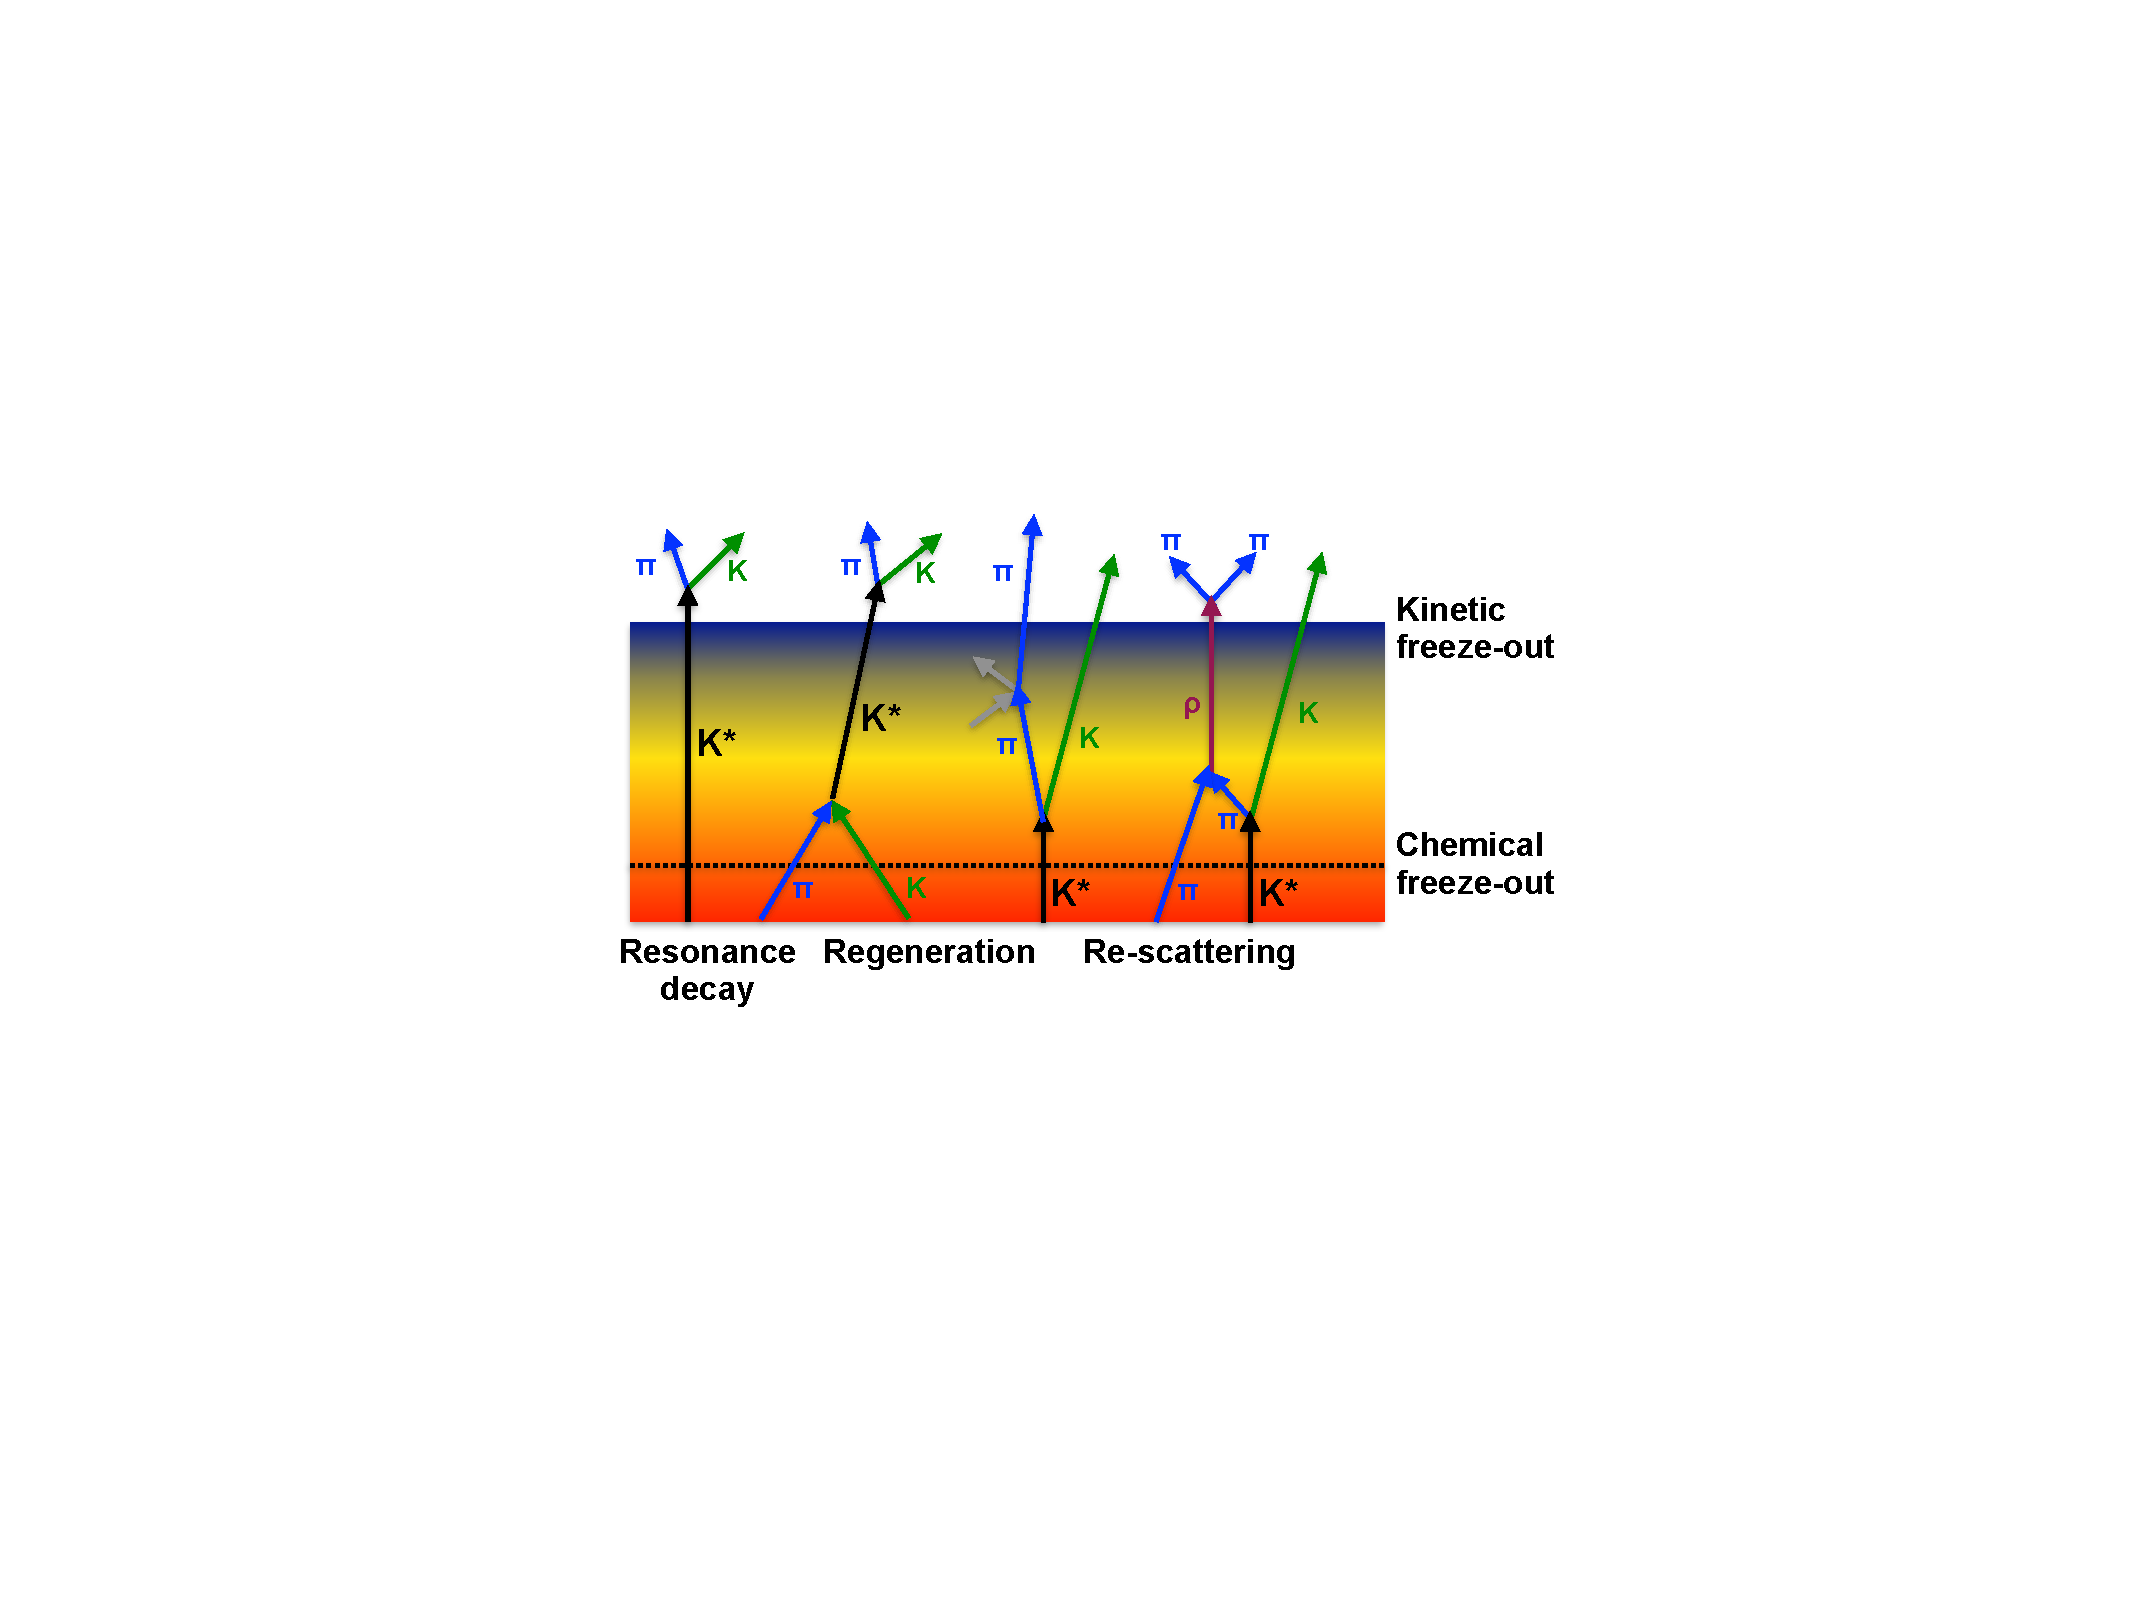
\includegraphics[width=12.cm]{./Version1/FigChapter3/Hadronic}
\caption{Hadronic phase }
\label{fig:hadronic}
\end{center}
\end{figure}



Resonances are particles with larger mass than the corresponding its ground state particle which has the same quark content. Because of the hadronic resonances decay strongly in the medium, it has short lifetime($\tau$) in the order of few fm/c which is comparable to the lifetime of the fireball. The natural width of resonances is given by $\Gamma = \bar{h}$/$\tau$, which is inversely proportion to the lifetime. 
In heavy-ion collisions, the hadronic resonances are produced in medium which is still expanding so that the particles could interact with the medium and decay while traveling it. The particles can be measured only via reconstruction of their decay products in a detector, since it decays very shortly after being produced.

The effects which can be happened in the hadronic phase is shown in Figure \ref{fig:hadronic}. In the left on the figure, as example, there is sketch of the original resonance decay of K*(892)$^{0}$ (K*(892)$^{0}$ $\rightarrow$ $\pi$+K). It is possible that resonances may be regenerated via pseudo-elastic scattering of decay products ( $\pi$+K $\rightarrow $ K*(892)$^{0}$ $\rightarrow$ $\pi$+K) in the time duration between the chemical ($T_{ch}$) and the kinetic freeze-out ($T_{kin}$).
Conversely, in case that the decay product undergo elastic scattering or pseudo-elastic scattering through a different resonance in the medium, e.g. $\rho$ in the Figure \ref{fig:hadronic}, the invariant mass of the daughters can not mach that of the parent particle. As a results, yield after kinetic freeze out could be smaller than the yields originally produced.

These re-scattering and regeneration depend on the lifetime of the resonances and affect the their yield and momentum spectrum. The yield is increase if the regeneration dominates, vice versa, it is decrease with re-scattering effect. In order to understand the properties in hadronic medium, the ratios between resonances and stable hadrons have to be studies and the results are compared with model predictions discussed in Section \ref{sec:model}.




\newpage